\documentclass[12pt]{article}
\usepackage{mathtools}
\usepackage{multicol}
\usepackage{float}
\usepackage[margin=1in]{geometry}
\usepackage{setspace}
\usepackage{mathrsfs}
\usepackage{gensymb}
\usepackage{fancyhdr}
\usepackage{graphicx}
\usepackage{indentfirst}
\usepackage{wrapfig} 

\begin{document}
\subsection*{\centering Group 4 - UAV Project Executive Summary}

The goal of the UAV Obstacle Course project was to simulate the flight of an unmanned aerial vehicle (UAV) to a series of way points through an obstacle course filled with cubes and hoops. The UAV’s flight was scored based on whether it hit all of the way points, went through any of the hoops, and if it hit any obstacles. Functions for plotting the UAV’s obstacle course were provided, as were the steering functions used to direct the UAV to the way points.

We decided the best way to approach this simulation was to assign separate functions for individuals to write and then troubleshoot the project together. We used GitHub to keep track of file updates. The functions we wrote were UAVContol, UAVFlyThrough, UAVFlyToWayPoint, UAVFlyWayPointSequence, stopSim, ODENumIntRK4 and UAVRHS. We modified PlotUAVObstacleCourse to run as well. The overarching structure of the simulation was provided to us, and which we followed. PlotUAVObstacleCourse takes in a way point list, initializes the state vector, control gains, UAV parameters, engine time response and then calls UAVFlyWaypointSequence. UAVFlyWaypointSequence loops through the waypoints, setting parameters for each segment between waypoints and calling UAVFlyToWayPoint. UAVFlyToWaypoint sets a time interval for the segment and calls UAVSim. UAVSim calls UAVGuidance, which calculates the required state for the UAV to get to the next waypoint. UAVControl took the current state, commanded state and gain parameters and output the required bank angle, normalized lift, and normalized thrust. UAVRHS is the dynamic model outputting the state derivatives, and is called after UAVControl inside UAVSim. The state is then updated and then the next time step is simulated. stopSim break’s UAVSim if it times out, which occurs when the UAV is incapable of reaching the waypoint due to control limits, or if the UAV passes through the waypoint. 

\begin{wrapfigure}{L}{0.5\textwidth}
	\begin{center}
		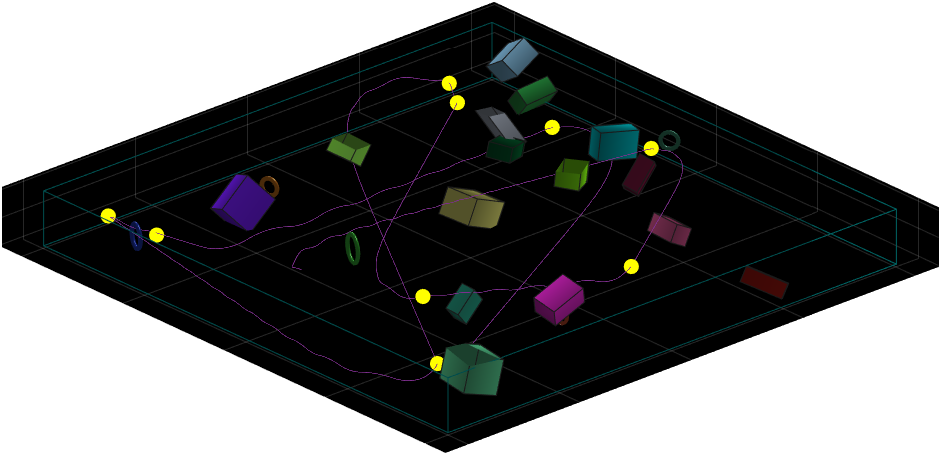
\includegraphics[scale=0.5]{Figure1}
		\caption{UAV Trajectory Through Course 1}
	\end{center}
\end{wrapfigure} 

Besides following the project instructions, we also added a few features to the simulation to make sure the UAV could get to each waypoint. Inside UAVControl, limits were applied to the bank angle, normalized lift and normalized thrust. Not only do those limits more accurately represent an actual flight, they made the simulation run smoother and kept the all values as real numbers. Adding additional waypoints made it easier for the UAV to fly to each required waypoint, as it wasn’t trying to turn quite so hard. In UAVRHS, limits were applied to the UAV to keep it within the boundaries of the obstacle course. 

Figure 1 shows the simulation of the UAV through Course 1 with additional waypoints. Running the course through the scoring function obtains an overall score of 1000 points. The UAV makes it through 2 hoops, but hits 6 cuboids. 	




\pagebreak
\subsection*{\centering Summary of Roles}  

\begin{description}
\item[Julia Dunlop:] Wrote the UAVControl and added limits to UAVRHS to keep UAV inside course. Wrote the majority of the executive summary. 

\item[Zixin Chen:] Wrote the entire RHS function. Revised and made extra comments on the code.

\item[Peter Hartford:] Wrote the ODENumIntRK4 function, formatted the executive summary, and published the MATLAB code. 

\item[Trevor Burgoyne:]
\end{description} 



\end{document}